\section{Experiments}
\label{sec:experiments}

\subsection{Experimental Setup}
\label{sec:setup}

\paragraph{Models.}
We evaluate nine models spanning seven architecture families and diverse attention configurations:
\textbf{Qwen2.5-7B} (GQA 7:1, 28 layers $\times$ 4 KV heads = 112),
\textbf{Qwen2.5-14B} (GQA 5:1, 48 $\times$ 8 = 384),
\textbf{Yi-1.5-9B} (GQA 8:1, 48 $\times$ 4 = 192),
\textbf{Llama-3.1-8B} (GQA 4:1, 32 $\times$ 8 = 256),
\textbf{CodeLlama-7B}\footnote{CodeLlama multi-bit profiles synthesized from 2-bit-only profiling; classification robust as constrained allocation is dominated by 4-bit heads.} (MHA 1:1, 32 $\times$ 32 = 1024),
\textbf{Mistral-7B-v0.3} (GQA 4:1, 32 $\times$ 8 = 256, sliding window attention),
\textbf{Gemma-2-9B} (GQA 2:1, 42 $\times$ 8 = 336, \texttt{head\_dim}=256, attention logit softcapping),
\textbf{Phi-3-medium-14B} (GQA 4:1, 40 $\times$ 10 = 400),
and \textbf{Pythia-1.4B} (MHA 1:1, 24 $\times$ 16 = 384).
All nine models undergo full constrained evaluation.
This selection spans GQA ratios from 1:1 (MHA) to 8:1 and covers standard, sliding-window, softcapped, and multi-head attention.

\paragraph{Evaluation.}
We report perplexity (PPL, $\downarrow$) on the WikiText-2 test split (298{,}938 tokens) under bf16 inference with stride 512.
For downstream evaluation, we use ARC-Challenge, HellaSwag, PIQA, and WinoGrande under 0-shot prompting.

\paragraph{Profiling.}
Per-head sensitivity is measured by independently quantizing each head to each candidate bit-width in $\{2, 4, 8, 16\}$ and recording the PPL increase over the bf16 baseline.
All results use high-resolution profiling (64 sequences $\times$ 2048 tokens from WikiText-2 train); Appendix~\ref{sec:profiling_resolution} compares against standard-resolution profiling (16 seq $\times$ 512 tok).

\paragraph{Compression and constraint.}
The default target is 4$\times$ compression (average 4 bits, budget ratio 0.25).
The cardinality constraint limits 2-bit assignments to at most $k$ heads, where $k$ is selected via the compounding sweep described in \S\ref{sec:method} ($k{=}8$ for Qwen-7B and Qwen-14B, $k{=}2$ for Yi-1.5, Llama, CodeLlama, and Mistral, $k{=}8$ for Gemma-2, Phi-3-medium, and Pythia).

\paragraph{Baselines.}
We compare against:
(1)~uniform 4-bit quantization;
(2)~unconstrained greedy allocation (RateQuant-style~\cite{zuo2026ratequant});
(3)~unconstrained MCKP allocation;
(4)~an L0-random heuristic that assigns Layer-0 heads to 8-bit and $k$ random non-Layer-0 heads to 2-bit, with remaining heads at 4-bit (5 seeds; we report mean$\pm$std and median);
and (5)~a naive positional heuristic that assigns Layer-0 to 8-bit and the $k$ deepest heads to 2-bit.

\subsection{Main Results}
\label{sec:main_results}

\begin{table}[t]
\centering
\small
\caption{PPL ($\downarrow$) on WikiText-2 at 4$\times$ compression. Unconstrained failure: catastrophic on Qwen-7B ($3.3\times$ bf16), severe on Pythia ($1.9\times$), moderate on Gemma-2 ($1.5\times$), mild on remaining incl.\ Qwen-14B (${\sim}1.1\times$). Greedy and MCKP columns are both unconstrained; identical allocations on 6/8 models (equivalence verified experimentally on Qwen-7B and Qwen-14B; Qwen-14B and Pythia Greedy values inferred via this equivalence). Best constrained result per model in \textbf{bold}. $^*$BOS-corrected.}
\label{tab:main_results}
\begin{tabular}{lccccc}
\toprule
Model & Baseline & Uniform & \multicolumn{2}{c}{Unconstrained} & Ours \\
\cmidrule(lr){4-5}
 & (bf16) & (4-bit) & Greedy & MCKP & (Constr.) \\
\midrule
Qwen2.5-7B      & 9.81  & 15.45 & 32.45 & 36.92 & \textbf{10.91} \\
Qwen2.5-14B     & 6.87  & 7.20  & 7.69  & 7.69  & 7.22 \\
Yi-1.5-9B       & 7.02  & 7.22  & 7.56  & 7.56  & 7.22 \\
Llama-3.1-8B    & 8.09  & 8.47  & 8.63  & 8.63  & \textbf{8.45} \\
Mistral-7B-v0.3 & 7.04  & 7.13  & 7.57  & 7.60  & 7.13 \\
Gemma-2-9B$^*$  & 6.03  & 6.17  & 8.85  & 8.85  & 6.20 \\
Phi-3-medium-14B & 5.64 & 5.80  & 6.07  & 6.07  & 5.81 \\
Pythia-1.4B     & 16.49 & 24.29 & 31.54 & 31.54 & 24.45 \\
\bottomrule
\end{tabular}
\end{table}

On Qwen2.5-7B, constrained MCKP achieves 10.91 PPL, a 29.4\% reduction over uniform 4-bit (15.45).
Without the constraint, both greedy (32.45) and MCKP (36.92) perform \emph{worse} than uniform---a catastrophic failure from excessive 2-bit assignments compounding across layers.
Across 3 calibration seeds, constrained MCKP yields mean PPL 10.99$\pm$0.06 with 90.2\% three-way allocation agreement, confirming profiling stability.

On Llama-3.1-8B, the result is essentially indistinguishable from uniform (8.45 vs.\ 8.47, $\Delta < 0.02$ PPL).
Hires profiling reveals concentration $0.57$ (comparable to Qwen's $0.61$) but a spike pattern ($t_1/t_5{=}0.85$) dominated by a single head (L2H5), leaving no cross-bitwidth gradient to exploit.

On Yi-1.5-9B, constrained MCKP ($k{=}2$) matches uniform (7.22); despite high concentration (0.71), sensitivity is dominated by a single outlier (L4H3, $t_1/t_5{=}0.90$), a spike pattern with no cross-bitwidth gradient.
On Mistral-7B-v0.3, constrained MCKP ($k{=}2$) matches uniform (7.13 vs.\ 7.13); near-zero sensitivity differences and sliding-window attention leave no room for reallocation gains.

On Gemma-2-9B$^*$ (GQA 2:1), constrained MCKP ($k{=}8$) achieves 6.20 PPL vs.\ uniform 6.17 ($+$0.4\%).
Despite flat sensitivity (concentration 0.23), unconstrained MCKP degrades to 8.85 ($1.47\times$ bf16) from 31.5\% 2-bit over-allocation; the constraint reduces this to 8 heads, confirming universal over-allocation prevention.

On Phi-3-medium-14B (GQA 4:1), constrained MCKP ($k{=}8$) achieves 5.81 PPL vs.\ uniform 5.80, consistent with its flat sensitivity profile (concentration 0.17); unconstrained MCKP degrades mildly to 6.07 ($1.08\times$ bf16). %exp_id=phi3_medium_constrained_mckp

Unconstrained failure severity tracks heterogeneity shape: \emph{catastrophic} on Qwen-7B ($3.3\times$ bf16, 60\% heads at 2-bit), \emph{severe} on Pythia ($1.9\times$), \emph{moderate} on Gemma-2 ($1.47\times$), and \emph{mild} on remaining models (${\sim}1.07$--$1.12\times$) including Qwen-14B ($1.12\times$, 20\% 2-bit)---the within-family contrast directly reflects shape (spread vs.\ flat).
The additive distortion assumption underlying standard MCKP formulations systematically fails at these bit-width gaps.

\paragraph{Aggressive compression.}
At higher compression (5.3$\times$), the cardinality constraint becomes valuable even for non-spread models: on Llama, constrained MCKP reduces PPL from 2643.8 (uniform 2-bit) to 57.6 (45$\times$ improvement); on Mistral, from 519.1 to 11.9 (44$\times$ improvement). The constraint's universal value emerges at aggressive compression ratios where uniform low-bit becomes insufficient (Appendix~\ref{sec:budget_sweep}).

See Appendix~\ref{sec:allocation_appendix} (allocation visualization) and Appendix~\ref{sec:budget_sweep} (budget sweep) for additional detail.

MCKP consistently outperforms random L0-constrained allocation and naive positional baselines across all three tested models (median gap 5--16\%; Table~\ref{tab:heuristic} in Appendix~\ref{sec:heuristic_appendix}).

\paragraph{Comparison with KIVI.}
KIVI~\cite{liu2024kivi} uses asymmetric per-channel quantization with per-token scaling, applied uniformly across all heads.
At 4-bit ($r{=}0$), KIVI achieves near-lossless PPL (9.91 on Qwen, 8.14 on Llama vs.\ 9.81/8.09 bf16), while our symmetric scheme yields 15.45 and 8.47---a gap from the quantization method, not allocation.
Within the symmetric scheme, constrained MCKP reduces Qwen from 15.45 to 10.91 ($-$4.54 PPL) by reallocating bits across heads; on Llama (spike), the gain is negligible ($-$0.02).
The two approaches are orthogonal and composable: KIVI selects the per-channel scheme, our method selects the per-head bit-width.
However, composability does not imply additive benefit: on Qwen, KIVI+MCKP achieves 9.90 PPL---identical to KIVI alone (9.90; MCKP alone: 10.91), as the per-channel method subsumes the head-level reallocation signal.
Per-head allocation provides independent value in symmetric-only deployment environments---common in hardware accelerators that lack per-channel asymmetric support---where it is the sole degree of freedom for exploiting sensitivity heterogeneity.

% BEGIN BRANCH-A (kivi-compounding-persists)
% Under KIVI-style per-channel asymmetric quantization, unconstrained head-level
% allocation still exhibits compounding: PPL rises from $\mathrm{X}$ at $k{=}2$
% to $\mathrm{Y}$ at $k{=}64$, a $\mathrm{Z}{\times}$ super-linear degradation.
% The cardinality constraint reduces this to $\mathrm{W}$, confirming that
% compounding is driven by bit-width gaps rather than quantization
% scheme---the constraint provides independent value even when per-channel
% information is available.
% END BRANCH-A

% BEGIN BRANCH-B (kivi-compounding-disappears)
% Under KIVI-style per-channel asymmetric quantization, unconstrained allocation
% no longer exhibits catastrophic compounding (PPL $\mathrm{X}$ at $k{=}64$ vs
% $\mathrm{Y}$ at $k{=}2$, only $\mathrm{Z}{\times}$ increase). Per-channel
% scaling effectively absorbs the inter-head distortion that causes symmetric
% compounding. This confirms that the cardinality constraint's primary value lies
% in symmetric-only deployment environments where per-channel scaling is
% unavailable.
% END BRANCH-B

\subsection{Cross-Architecture Compounding}
\label{sec:compounding_cross}

\begin{figure}[t]
\centering
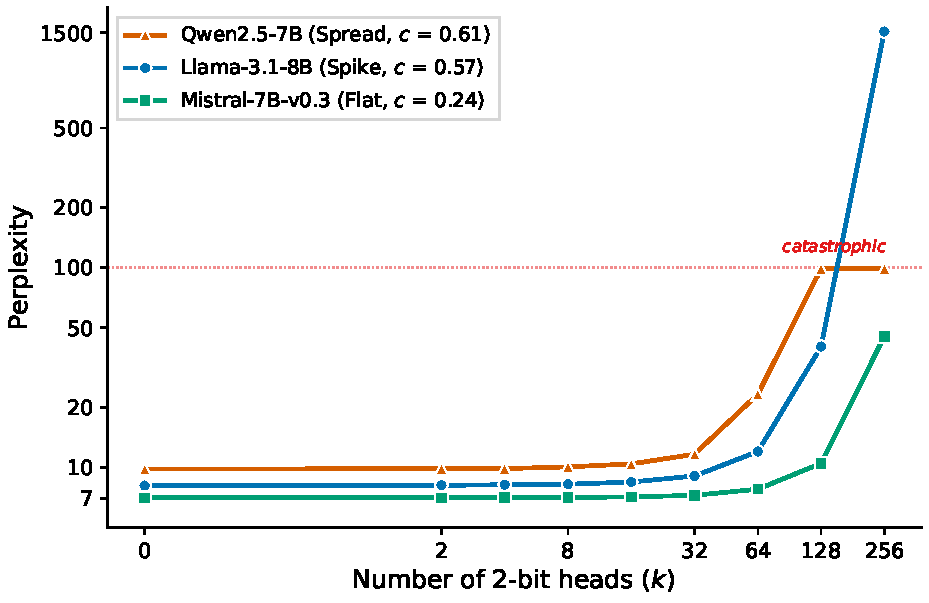
\includegraphics[width=\columnwidth]{figures/fig_compounding_curves.pdf}
\caption{Compounding effect across architectures. As the number of 2-bit heads ($k$) increases, PPL degradation follows architecture-dependent trajectories: Llama (spike, $c{=}0.57$) explodes to $188\times$ baseline (PPL 1519) at $k{=}256$ due to a single extreme-sensitivity head compounding through the residual stream; Qwen (spread, $c{=}0.61$) degrades $10\times$; Mistral (flat, $c{=}0.24$) remains most resilient ($6.4\times$). All three stay near-baseline for $k{\leq}8$, validating the cardinality constraint regime. Qwen saturates at $k{\approx}96$ due to its 112 KV heads (maximum ${\sim}96$ eligible for 2-bit assignment).}
\label{fig:compounding_cross}
\end{figure}

Figure~\ref{fig:compounding_cross} shows the compounding sweep across three architectures representing the three sensitivity patterns.
At small $k$ (${\leq}8$), all models tolerate 2-bit assignments with minimal PPL increase (${\leq}2.5\%$ over baseline), confirming that the cardinality constraint ($k{=}2$--$8$) operates in the near-additive regime regardless of architecture.

Beyond $k{=}8$, divergence is stark.
Llama (spike pattern) remains stable through $k{=}32$ (PPL $9.05$, $1.12\times$ baseline) but explodes at $k{=}128$ ($40.21$) and $k{=}256$ ($1519$, $188\times$ baseline)---the single extreme-sensitivity head (L2H5) amplifies compounding once enough surrounding heads are also degraded.
This binary failure mode---stable until the critical head is corrupted, then catastrophic---is analogous to critical-node failure in sparse networks.
Qwen (spread pattern) rises earlier, reaching $23.22$ at $k{=}64$ ($2.4\times$) and $98.75$ at $k{=}256$ ($10.1\times$), as its cluster of Layer-0 sensitive heads compound non-additively at moderate $k$.
At $k{=}64$, the observed PPL exceeds the additive prediction by $4.89\times$, confirming severe super-additivity.
Mistral (flat pattern) is the most resilient: PPL stays below $8$ through $k{=}64$ and reaches only $45.28$ at $k{=}256$ ($6.4\times$), consistent with its near-uniform sensitivity distribution offering no single failure mode.

These curves directly motivate architecture-specific $k$ selection: the compounding onset ($k$ at which PPL exceeds $1.5\times$ baseline) is ${\sim}32$ for Qwen, ${\sim}64$ for Llama, and ${\sim}128$ for Mistral, with the optimal constrained $k$ lying well below each onset.

\subsection{Downstream Evaluation}
\label{sec:downstream}

\begin{table}[t]
\centering
\small
\caption{0-shot accuracy change (Ours $-$ Uniform, pts) at 4$\times$ compression. Qwen values are mean over 3 calibration seeds ($\pm$1$\sigma$). Qwen shows gains on HS/PIQA/WG; the remaining models show near-neutral change, tracking PPL results.}
\label{tab:downstream}
\begin{tabular}{lccccc}
\toprule
Model & ARC-C & HS & PIQA & WG & Avg \\
\midrule
Qwen2.5-7B        & $+$0.0{\scriptsize$\pm$0.4} & $+$4.1{\scriptsize$\pm$0.2} & $+$2.0{\scriptsize$\pm$0.2} & $+$1.6{\scriptsize$\pm$1.2} & $+$1.9 \\
Yi-1.5-9B        & $-$2.1 & $-$0.4 & $+$0.0 & $+$0.3 & $-$0.5 \\
Llama-3.1-8B     & $-$0.8 & $+$0.0 & $-$0.1 & $+$0.5 & $-$0.1 \\
Mistral-7B       & $+$0.0 & $+$0.0 & $-$0.1 & $-$0.1 & $+$0.0 \\
Gemma-2-9B       & $-$0.1 & $+$0.0 & $+$0.4 & $+$0.6 & $+$0.2 \\
\bottomrule
\end{tabular}
\end{table}

On Qwen, constrained MCKP improves average 0-shot accuracy by 1.9 pts over uniform (mean over 3 seeds, $\pm$1$\sigma$ in Table~\ref{tab:downstream}), with the largest gains on HellaSwag ($+$4.1) and PIQA ($+$2.0).
The four non-spread models show near-neutral average change (Yi $-$0.5, Llama $-$0.1, Mistral $+$0.0, Gemma-2 $+$0.2 pts); Mistral is effectively unchanged across all tasks, consistent with its flat sensitivity profile.
ARC-Challenge shows the largest per-task sensitivity across all models (Yi $-$2.1, Llama $-$0.8, Gemma-2 $-$0.1 pts), consistent with multi-step reasoning where KV cache errors accumulate across longer inference chains.
Cross-dataset evaluation (Appendix~\ref{sec:cross_dataset}, ${>}96\%$ bit-assignment agreement across WikiText-2/C4) confirms calibration robustness.
Long-context evaluation (Appendix~\ref{sec:long_context}) reveals that the spread-pattern advantage amplifies with sequence length: on Qwen (spread), uniform 4-bit degrades from $1.57\times$ bf16 at 2K to $11.15\times$ at 8K, while constrained MCKP remains stable ($1.11\times$ to $1.23\times$).
In contrast, all three non-spread models show no benefit or slight degradation at 8K.
Llama-3.1-8B (spike, $t_1/t_5{=}0.85$): uniform $1.08\times$ bf16, MCKP $1.08\times$---identical.
Mistral-7B (flat, $c{=}0.24$): uniform $1.02\times$ bf16, MCKP $1.02\times$---identical.
Yi-1.5-9B (spike, $c{=}0.71$, $t_1/t_5{=}0.90$): uniform $1.05\times$ bf16, MCKP $1.06\times$---no benefit or slight degradation ($+$0.06~PPL), consistent with spike classification.
The uniform-to-constrained PPL ratio on Qwen widens from $1.4\times$ at 2K to $9.1\times$ at 8K, while Llama, Mistral, and Yi remain flat---long-context stress amplifies the spread-specific benefit of per-head allocation.
We note that Qwen-7B also has the fewest KV heads (112) in our test set; whether the long-context amplification is driven by the spread pattern, the low head count, or their interaction remains an open question requiring evaluation on additional spread-pattern models.